\documentclass[11pt,a4paper]{article}

\usepackage[utf8]{inputenc}
\usepackage[T1]{fontenc}
\usepackage{lmodern}
\usepackage[margin=2.5cm]{geometry}
\usepackage{booktabs}
\usepackage{tabularx}
\usepackage{array}
\usepackage{enumitem}
\usepackage{caption}
\usepackage{float}
\usepackage{graphicx}
\usepackage[round]{natbib}
\setcitestyle{citesep={,}}
\usepackage[hidelinks]{hyperref}

\newcolumntype{L}[1]{>{\raggedright\arraybackslash}p{#1}}
\setlength{\parskip}{4pt}
\setcounter{tocdepth}{2}
\graphicspath{{../figures/}}

\begin{document}

% ------------------------------------------------------------------
% TITLE PAGE
% ------------------------------------------------------------------

\begin{titlepage}
    \centering
    \vspace*{2cm}

    {\Large Vrije Universiteit Amsterdam\par}
    \vspace{0.4cm}

    {\large Subjectivity Mining, 2026 edition\par}
    \vspace{0.2cm}

    {\large Lecturers Isa Maks and Ilia Markov\par}

    \vspace{3.5cm}

    {\huge\bfseries Assignment 4\par}
    \vspace{0.5cm}

    {\LARGE Offensive language detection in in-domain\\[0.2cm] and cross-domain settings\par}

    \vspace{3cm}

    {\Large Group 9\par}
    \vspace{0.8cm}

    {\large
    \begin{tabular}{l}
        Ines Casado Vela \\
        Martin Ranea Marina \\
        Pablos Tselioudis Garmendia \\
        Helian X. Liu \\
    \end{tabular}\par}

    \vfill

    {\large 4 October 2026\par}

\end{titlepage}

\tableofcontents
\newpage

\noindent\textit{Content warning. This report discusses and quotes offensive language.}

% ------------------------------------------------------------------
\section{Introduction}
% ------------------------------------------------------------------

Models that detect offensive language are usually tested on data from the same dataset they were trained on. In real use, this is rarely the case. A model trained on one set of posts is often used on posts from another platform or about other topics, and then its scores tend to go down \citep{swamy2019studying,fortuna2021how}.

This report studies that problem with two English datasets, OLID and HASOC. Four models are compared. The first is a simple baseline, Logistic Regression with TF-IDF features. The other three are transformer models. One is the general BERT model, and the other two, HateBERT and fBERT, are versions of BERT that were trained further on offensive social media text. Each model is trained twice, once on OLID and once on HASOC. Both versions are then tested on the same OLID test set.

There are two goals. The first is to find out which model works best when the training and test data come from the same dataset. The second is to measure how much each model loses when they do not, and to explain why.

% ------------------------------------------------------------------
\section{Data}
% ------------------------------------------------------------------

\subsection{Sources}

The Offensive Language Identification Dataset, OLIDv1, has 14,100 English tweets \citep{zampieri2019olid}. Each tweet is labelled on three levels. The dataset was used in OffensEval 2019, which was SemEval 2019 Task 6 \citep{zampieri2019semeval}. This report only uses the first level, Subtask A. Here a tweet is offensive if it contains swearing or an attack on someone, such as an insult or a threat. The tweets were collected by searching for keywords, many of them political, and they were labelled by crowd workers. User names are replaced by @USER and links by URL.

HASOC comes from a shared task on hate speech and offensive content at FIRE 2019 \citep{mandl2019hasoc}. Only the English training set is used. It contains posts from both Twitter and Facebook. Its positive class, called HOF, puts hate speech together with offensive and profane posts. The posts were collected with hashtags and keywords about events in 2019, so the topics are very different from OLID. Also, HASOC does not hide user names.

The course gave preprocessed versions of both datasets. In all of them, label 1 means offensive and label 0 means non-offensive. The file olid-train-small is a part of the OLID training data. It was picked so that it has the same size and the same label balance as the HASOC training set. The test set is the original OffensEval 2019 test set.

\subsection{Statistics}

Table~\ref{tab:data-stats} shows the main statistics. The two training sets have the same size and the same label balance. Each has 5,852 messages, and 38.6 percent of them are offensive. This was done on purpose. Because of it, any difference between the in-domain and cross-domain results cannot come from more training data or a different label balance.

\begin{table}[H]
\centering
\caption{Statistics of the three datasets. Word counts use whitespace splitting. WordPiece counts use the uncased BERT tokenizer and include the two special tokens.}
\label{tab:data-stats}
\begin{tabular}{lrrrrrrr}
\toprule
 & & & & & \multicolumn{3}{c}{Mean length} \\
\cmidrule(lr){6-8}
Dataset & Messages & Class 0 & Class 1 & Off. \% & Words & Chars & WordPieces \\
\midrule
OLID train small & 5,852 & 3,591 & 2,261 & 38.6 & 22.4 & 126.3 & 33.7 \\
HASOC train      & 5,852 & 3,591 & 2,261 & 38.6 & 23.3 & 167.0 & 47.4 \\
OLID test        & 860   & 620   & 240   & 27.9 & 24.4 & 146.1 & 40.3 \\
\bottomrule
\end{tabular}
\end{table}

The test set is less balanced than the training sets. Only 27.9 percent of the test tweets are offensive. A model that predicts the offensive class too often will therefore make many false positives.

The difference in length depends on how it is measured. In words, HASOC messages are only about one word longer than OLID messages. In characters they are about a third longer, and in WordPieces, the sub-word units BERT works with, they are 40 percent longer. This comes from long hashtags and real user names, which add many characters but few normal words. The transformers cut messages off after 128 tokens. This only happens to 14 messages in OLID train small and 11 in HASOC, and never in the test set.

\subsection{Domain differences}

To show how the datasets differ, some simple properties were counted in each of them. Table~\ref{tab:domain} shows the results.

\begin{table}[H]
\centering
\caption{Simple properties of the datasets, in percent of messages unless stated otherwise. Explicit words are found with a short list of about 25 swear words and insults. Coverage is the share of OLID test words, counted as tokens or as unique words, that also appear in the training set.}
\label{tab:domain}
\begin{tabular}{lrrr}
\toprule
Property & OLID train small & HASOC train & OLID test \\
\midrule
Contains the @USER placeholder & 92.7 & 0.0 & 38.5 \\
Contains a real user handle & 0.0 & 51.5 & 0.0 \\
Contains the URL placeholder & 14.1 & 0.0 & 55.9 \\
Contains at least one hashtag & 14.2 & 98.4 & 73.8 \\
Hashtags per message, mean & 0.4 & 3.2 & 2.3 \\
Explicit word, offensive messages & 31.0 & 45.6 & 36.7 \\
Explicit word, non-offensive messages & 2.8 & 27.4 & 2.7 \\
Test token coverage & 89.1 & 81.6 & \\
Test word type coverage & 62.0 & 58.1 & \\
\bottomrule
\end{tabular}
\end{table}

The table shows four main differences. First, the datasets are formatted differently. OLID replaces users and links with placeholders. HASOC keeps the real user names, and almost every HASOC post has hashtags. So a model trained on HASOC has never seen the @USER token, even though it appears in more than a third of the test tweets.

Second, the topics are different. The most common words in OLID train small are gun, liberals, antifa, MAGA and conservatives, which are all about American politics in 2018. HASOC is full of hashtags like fucktrump, trumpisatraitor, shameonicc, dhonikeepstheglove and doctorsfightback. These are about Trump, the 2019 Cricket World Cup, a doctors' strike in India and the race to replace Theresa May. The word overlap shows this too. OLID train small contains 89.1 percent of the words in the test set, HASOC only 81.6 percent.

Third, and probably most important, swear words are labelled differently in the two datasets. In OLID, only 2.8 percent of the non-offensive messages contain a swear word or insult. In HASOC this is 27.4 percent. Many HASOC posts with words like fuck, for example inside a hashtag, are still labelled non-offensive. So in HASOC, swearing is a much weaker sign of the offensive label, and a model trained on HASOC learns a different idea of what offensive means.

Finally, the OLID test set is also a bit different from OLID train small. It has many more hashtags and URL placeholders. This suggests that its tweets were collected in a slightly different way. So even the in-domain setting has a small domain shift.

A quick check of the data found some smaller problems. Each file has some duplicate texts, 8 in OLID train small, 78 in HASOC and 11 in the test set. Also, three test tweets appear in exactly the same form in OLID train small. One test tweet only says NAME with a question mark, which is a typical spreadsheet error, and it is labelled offensive. These cases were kept, so that all models use exactly the files that were given.

% ------------------------------------------------------------------
\section{Experimental setup}
% ------------------------------------------------------------------

Every model is run in two settings.

\textbf{In-domain.} The model is trained on olid-train-small and tested on olid-test. Training and test data come from the same dataset.

\textbf{Cross-domain.} The model is trained on hasoc-train and tested on the same olid-test file.

The test set is the same in both settings, so the only thing that changes is the training data. The cross-domain model always starts from the original pre-trained model, never from the in-domain model. The test set is never used for training or tuning. No development set is needed either, because no model had its hyperparameters tuned.

All models are scored with the same evaluation function from the shared notebook. It gives accuracy, macro-averaged precision, recall and F1, the same three scores for each class, and the confusion matrix. Macro-F1 is the main score. Only 28 percent of the test tweets are offensive, so accuracy mostly shows how well a model does on the larger class. Macro-F1 gives both classes the same weight. The drop from in-domain to cross-domain is given in macro-F1 points and as a percentage of the in-domain score.

The in-domain and cross-domain predictions of each model are also compared with an exact McNemar test \citep{mcnemar1947note}. Both models predict the same 860 tweets, so this test shows whether the change in errors is bigger than what chance alone would give.

% ------------------------------------------------------------------
\section{Methods}
% ------------------------------------------------------------------

\subsection{Overview}

Four models are compared. Logistic Regression with TF-IDF features is the simple baseline. It only looks at which words appear in a message. The three transformer models all have the same BERT base structure, with 12 layers and about 110 million parameters. They differ in the text they were pre-trained on. BERT is the general model \citep{devlin2019bert}. HateBERT and fBERT start from BERT and are then trained further on offensive or abusive social media text. Comparing them shows if this extra training helps, especially when the training data comes from another dataset.

All transformer models are fine-tuned with the Simple Transformers library \citep{rajapakse2019simpletransformers}. The library puts a classification layer on top of the model and then trains all the weights on the labelled data. The predicted label is the class with the highest score. Table~\ref{tab:hyper} lists the settings of each model.

\begin{table}[H]
\centering
\caption{Model checkpoints and training settings. All transformer runs fine-tune for 3 epochs, which is 1,098 optimiser steps with an effective batch size of 16, and use the AdamW optimiser with a linear learning rate schedule and 6 percent warmup. None uses class weights.}
\label{tab:hyper}
\footnotesize
\setlength{\tabcolsep}{4pt}
\begin{tabular}{L{2.1cm}L{3.0cm}L{2.85cm}L{2.85cm}L{2.85cm}}
\toprule
 & Logistic Regression & BERT & HateBERT & fBERT \\
\midrule
Checkpoint & none & bert-base-cased & GroNLP\slash hateBERT & diptanu\slash fBERT \\
Casing & lowercased & cased & uncased & uncased \\
Features & word 1 and 2 grams, TF-IDF, min df 2, max 50,000, sublinear tf & WordPiece, max 128 tokens & WordPiece, max 128 tokens & WordPiece, max 128 tokens \\
Learning rate & not applicable & 4e-5 & 2e-5 & 2e-5 \\
Weight decay & L2, C = 1 & 0 & 0.01 & 0.01 \\
Batch size & full data & 16 & 8, with 2 accumulation steps & 8, with 2 accumulation steps \\
Precision & not applicable & FP16 & FP16 & FP16 \\
Class weights & balanced & none & none & none \\
Seed & 42 & 42 & 42 & 42 \\
Hardware & CPU & Google Colab GPU & RTX 4060 laptop GPU & RTX 4070 laptop GPU \\
\bottomrule
\end{tabular}
\end{table}

\subsection{Logistic Regression baseline}

The baseline is built with scikit-learn \citep{pedregosa2011scikit}. Each message is put in lowercase and turned into TF-IDF weights of single words and word pairs. Words that appear in fewer than two training messages are left out, and at most 50,000 features are kept. Logistic Regression is used with balanced class weights. This means that mistakes on the smaller offensive class count more during training. The TF-IDF vocabulary is built only from the training set of each setting. In the cross-domain run, the model therefore only knows words that appear in HASOC.

\subsection{BERT}

BERT was pre-trained on English books and Wikipedia \citep{devlin2019bert}. The cased version is used here, which keeps capital letters. This can help with tweets, where words in capitals often mean shouting. The model is trained for 3 epochs with a batch size of 16, a learning rate of 4e-5 and a maximum length of 128 tokens. All other settings are the Simple Transformers defaults, so there is no weight decay, 6 percent warmup and mixed precision. The training was done on a Google Colab GPU.

\subsection{HateBERT}

HateBERT is the uncased BERT base model, trained further on RAL-E \citep{caselli2021hatebert}. RAL-E has about 1.5 million Reddit messages from communities that were banned for abusive or hateful content. The HateBERT model is a language model and not a classifier, so its classification layer starts from scratch. The training settings were chosen before any test results were seen. Compared with BERT, the learning rate is lower, 2e-5, and a weight decay of 0.01 is used. A batch of 8 with two accumulation steps gives the same effective batch size of 16. The exact model version and all settings are saved in the run files in the notebook folder.

\subsection{fBERT}

fBERT is also the uncased BERT base model, but it was trained further on more than 1.4 million offensive tweets from SOLID \citep{sarkar2021fbert}. SOLID is a very large dataset built as an extension of OLID \citep{rosenthal2021solid}. It uses the same labelling scheme, and its labels were made by models trained on OLID. This matters a lot for the results. Of all the models here, fBERT is the one whose pre-training data is closest to the test data.

To compare fBERT fairly with HateBERT, fBERT uses exactly the same code and settings as HateBERT. Only the model name is changed. The fBERT checkpoint does not include the weights of the pooling layer, so this layer and the classification layer both start from random weights. Each fBERT run took about 135 seconds on an RTX 4070 laptop GPU.

Results of a single training run can change with the random seed. For that reason, fBERT and HateBERT were also trained with two extra seeds, 1 and 2, in both settings. These extra runs are only used to check if the results are stable. All main tables show the runs with seed 42.

% ------------------------------------------------------------------
\section{Results}
% ------------------------------------------------------------------

\subsection{Overall performance}

Table~\ref{tab:overall} shows the macro-averaged scores of all models, and Figure~\ref{fig:macro} compares their macro-F1.

\begin{table}[H]
\centering
\caption{Accuracy and macro-averaged precision, recall and F1 on the OLID test set, 860 tweets. The best score per setting is in bold.}
\label{tab:overall}
\begin{tabular}{llrrrr}
\toprule
Model & Setting & Accuracy & Macro-P & Macro-R & Macro-F1 \\
\midrule
Logistic Regression & In-domain    & 0.7407 & 0.6861 & 0.7027 & 0.6923 \\
BERT                & In-domain    & 0.8209 & 0.7769 & 0.7864 & 0.7813 \\
HateBERT            & In-domain    & \textbf{0.8407} & \textbf{0.8022} & 0.8014 & 0.8018 \\
fBERT               & In-domain    & \textbf{0.8407} & 0.8014 & \textbf{0.8052} & \textbf{0.8033} \\
\midrule
Logistic Regression & Cross-domain & 0.5186 & 0.5572 & 0.5691 & 0.5094 \\
BERT                & Cross-domain & 0.7709 & 0.7177 & 0.7288 & 0.7226 \\
HateBERT            & Cross-domain & 0.8035 & 0.7560 & 0.7513 & 0.7536 \\
fBERT               & Cross-domain & \textbf{0.8547} & \textbf{0.8317} & \textbf{0.7932} & \textbf{0.8088} \\
\bottomrule
\end{tabular}
\end{table}

\begin{figure}[H]
\centering
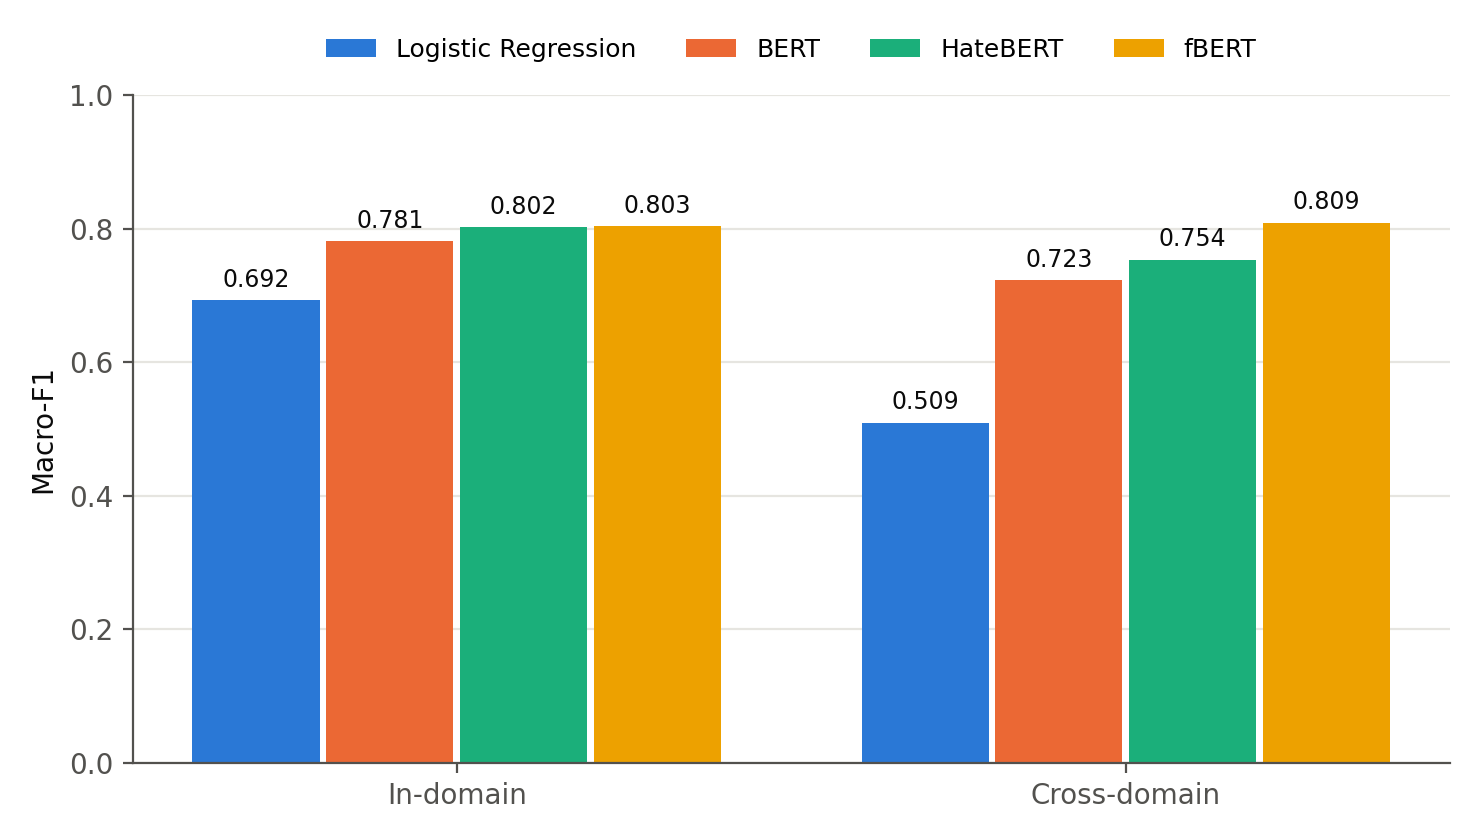
\includegraphics[width=0.8\linewidth]{macro_f1_all_models.png}
\caption{Macro-F1 of the four models in both settings, evaluated on the same OLID test set.}
\label{fig:macro}
\end{figure}

In the in-domain setting, all transformer models do much better than the baseline. BERT scores almost 9 macro-F1 points higher than Logistic Regression, and HateBERT and fBERT add another 2 points. fBERT has the highest in-domain macro-F1, 0.8033, but HateBERT is almost the same with 0.8018. They also have the same accuracy, and a McNemar test shows no real difference between them. Each model gets exactly 40 tweets right that the other gets wrong.

In the cross-domain setting the differences are much larger. Logistic Regression drops to a macro-F1 of 0.5094. Random guessing would give about 0.48 on this test set, so the baseline is only a little better than chance. BERT and HateBERT do much better but still lose points. fBERT behaves differently. Trained on HASOC, it scores 0.8088, which is the best cross-domain score and slightly higher than its own in-domain score.

\subsection{Per-class results}

Table~\ref{tab:perclass} shows the scores for each class, and Figure~\ref{fig:class} shows the F1 per class.

\begin{table}[H]
\centering
\caption{Precision, recall and F1 per class. Class 0 is non-offensive, 620 tweets. Class 1 is offensive, 240 tweets.}
\label{tab:perclass}
\begin{tabular}{llrrrrrr}
\toprule
 & & \multicolumn{3}{c}{Class 0, non-offensive} & \multicolumn{3}{c}{Class 1, offensive} \\
\cmidrule(lr){3-5}\cmidrule(lr){6-8}
Model & Setting & P & R & F1 & P & R & F1 \\
\midrule
Logistic Regression & In-domain    & 0.8417 & 0.7887 & 0.8143 & 0.5305 & 0.6167 & 0.5703 \\
BERT                & In-domain    & 0.8845 & 0.8645 & 0.8744 & 0.6693 & 0.7083 & 0.6883 \\
HateBERT            & In-domain    & 0.8889 & 0.8903 & 0.8896 & 0.7155 & 0.7125 & 0.7140 \\
fBERT               & In-domain    & 0.8927 & 0.8855 & 0.8891 & 0.7102 & 0.7250 & 0.7175 \\
\midrule
Logistic Regression & Cross-domain & 0.7877 & 0.4548 & 0.5767 & 0.3267 & 0.6833 & 0.4420 \\
BERT                & Cross-domain & 0.8531 & 0.8242 & 0.8384 & 0.5824 & 0.6333 & 0.6068 \\
HateBERT            & Cross-domain & 0.8596 & 0.8694 & 0.8645 & 0.6524 & 0.6333 & 0.6427 \\
fBERT               & Cross-domain & 0.8744 & 0.9323 & 0.9024 & 0.7889 & 0.6542 & 0.7153 \\
\bottomrule
\end{tabular}
\end{table}

\begin{figure}[H]
\centering
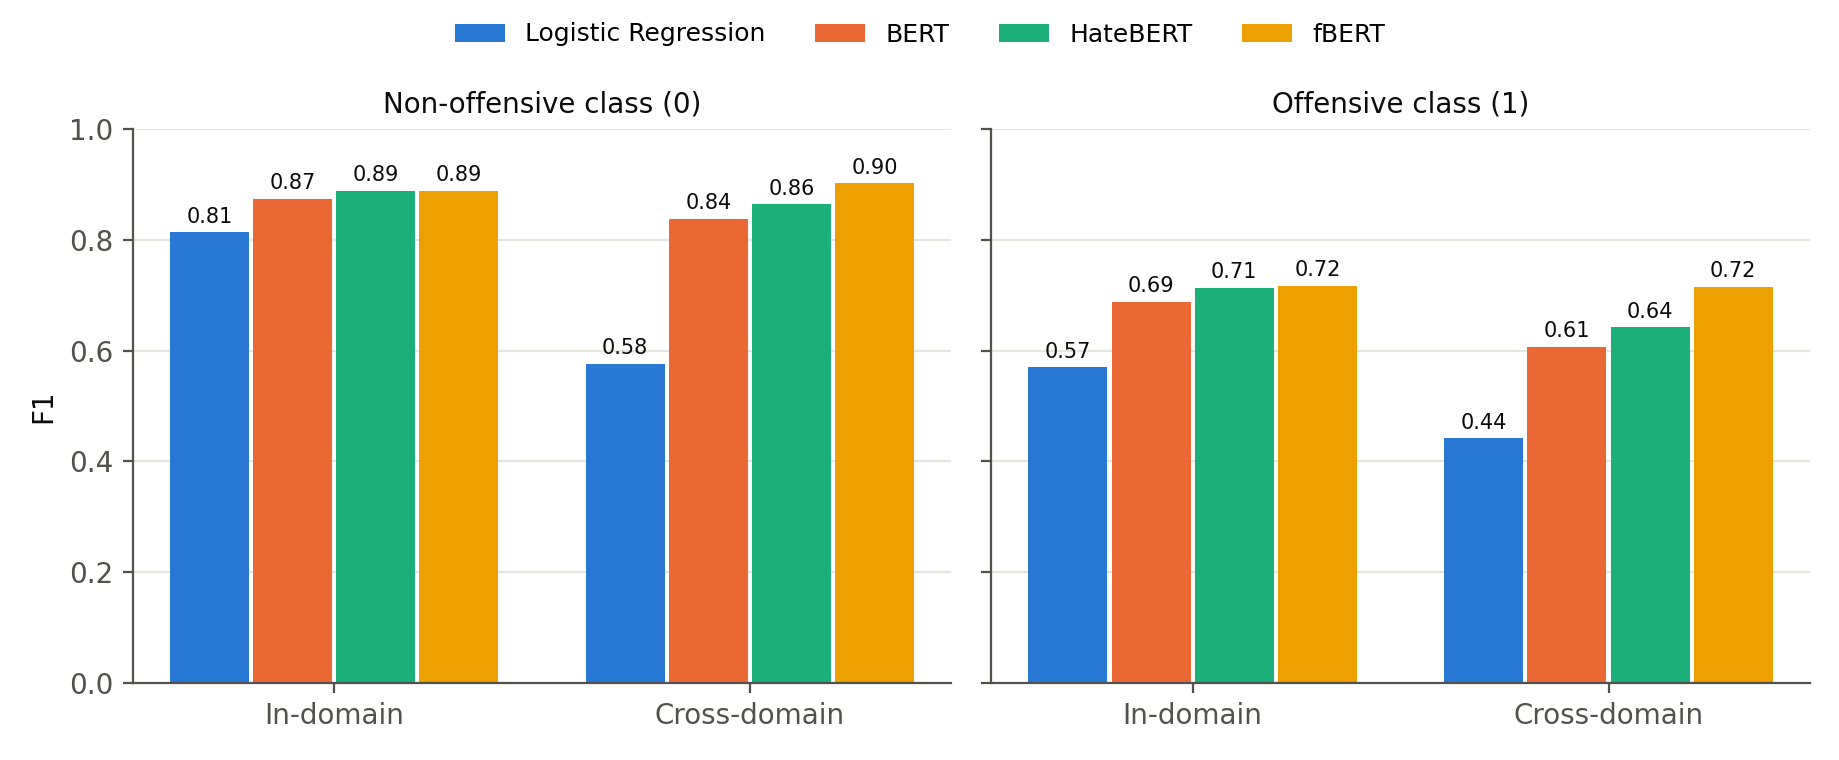
\includegraphics[width=0.95\linewidth]{class_f1_all_models.png}
\caption{F1 for the non-offensive class, left, and the offensive class, right.}
\label{fig:class}
\end{figure}

The offensive class is harder for every model in every setting. The best in-domain models reach about 0.72 F1 on it, compared with 0.89 on the non-offensive class. One reason is the class balance. There are fewer offensive examples to learn from, and with only 240 offensive test tweets, each false positive has a bigger effect on precision.

\subsection{Confusion matrices}

Figure~\ref{fig:cm} shows all eight confusion matrices, and Table~\ref{tab:errors} turns them into error rates.

\begin{figure}[H]
\centering
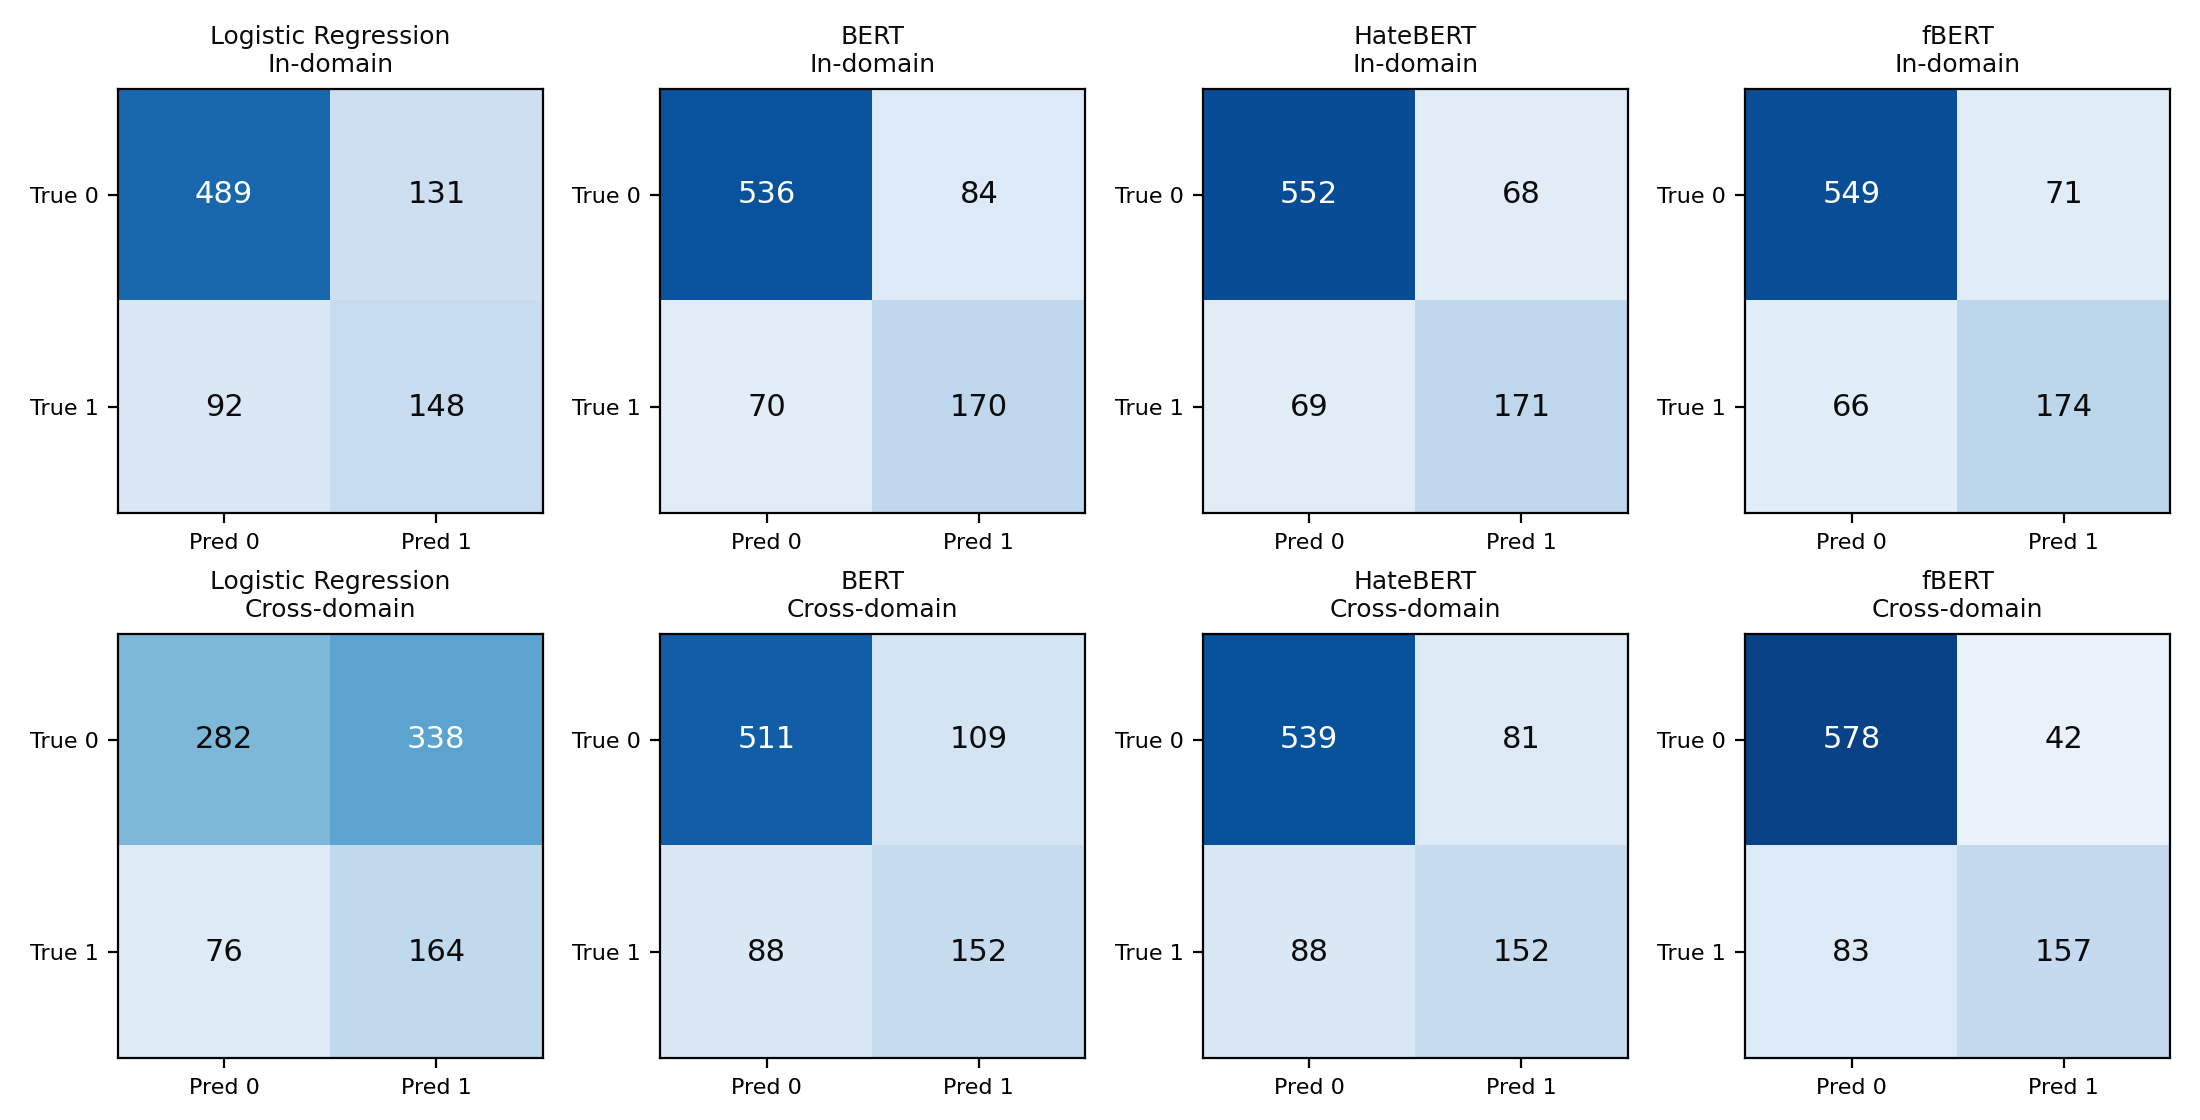
\includegraphics[width=\linewidth]{confusion_matrices_all.png}
\caption{Confusion matrices on the OLID test set. Rows are true labels and columns are predictions. Top row in-domain, bottom row cross-domain.}
\label{fig:cm}
\end{figure}

\begin{table}[H]
\centering
\caption{Error counts and rates. FPR is the share of non-offensive tweets predicted as offensive, FNR the share of offensive tweets predicted as non-offensive. The last column is the share of all test tweets predicted as offensive, the true value is 27.9 percent.}
\label{tab:errors}
\begin{tabular}{llrrrrr}
\toprule
Model & Setting & FP & FN & FPR & FNR & Predicted offensive \% \\
\midrule
Logistic Regression & In-domain    & 131 & 92 & 0.211 & 0.383 & 32.4 \\
BERT                & In-domain    & 84  & 70 & 0.135 & 0.292 & 29.5 \\
HateBERT            & In-domain    & 68  & 69 & 0.110 & 0.288 & 27.8 \\
fBERT               & In-domain    & 71  & 66 & 0.115 & 0.275 & 28.5 \\
\midrule
Logistic Regression & Cross-domain & 338 & 76 & 0.545 & 0.317 & 58.4 \\
BERT                & Cross-domain & 109 & 88 & 0.176 & 0.367 & 30.3 \\
HateBERT            & Cross-domain & 81  & 88 & 0.131 & 0.367 & 27.1 \\
fBERT               & Cross-domain & 42  & 83 & 0.068 & 0.346 & 23.1 \\
\bottomrule
\end{tabular}
\end{table}

The models make very different kinds of mistakes. When Logistic Regression is trained on HASOC, it labels 58 percent of the test tweets as offensive, which is more than twice the real rate. Its false positives go up from 131 to 338, so more than half of the harmless tweets are flagged. The transformer models do not do this. They predict about the right share of offensive tweets, and most of their extra errors are offensive tweets they miss. For BERT and HateBERT, the false negatives go up from about 70 to 88. fBERT becomes more careful instead. Trained on HASOC, it predicts too few tweets as offensive. Its false positives go down from 71 to 42, and its false negatives go up from 66 to 83.

% ------------------------------------------------------------------
\section{Analysis}
% ------------------------------------------------------------------

\subsection{Size of the cross-domain drop}

Table~\ref{tab:drop} shows how much each model changes from the in-domain to the cross-domain setting.

\begin{table}[H]
\centering
\caption{Change in macro-F1 and in offensive-class F1 from in-domain to cross-domain. Positive values are drops. The relative drop is in percent of the in-domain macro-F1. The McNemar p-value shows if the in-domain and cross-domain models make different errors on the same 860 tweets.}
\label{tab:drop}
\resizebox{\linewidth}{!}{%
\begin{tabular}{lrrrrrr}
\toprule
Model & Macro-F1 in & Macro-F1 cross & Absolute drop & Relative drop & F1 drop, class 1 & McNemar p \\
\midrule
Logistic Regression & 0.6923 & 0.5094 & 0.1830 & 26.4 & 0.1283 & $<$0.001 \\
BERT                & 0.7813 & 0.7226 & 0.0587 & 7.5  & 0.0815 & 0.001 \\
HateBERT            & 0.8018 & 0.7536 & 0.0482 & 6.0  & 0.0713 & 0.003 \\
fBERT               & 0.8033 & 0.8088 & $-$0.0055 & $-$0.7 & 0.0023 & 0.219 \\
\bottomrule
\end{tabular}}
\end{table}

Three of the four models drop. Logistic Regression loses 18.3 macro-F1 points, more than a quarter of its in-domain score. BERT loses 5.9 points and HateBERT 4.8. For these models, the McNemar test shows that the drop is not due to chance.

fBERT does not drop. Its cross-domain score is 0.6 points higher. The McNemar test gives p = 0.22, so there is no significant difference between its two versions. To make sure this is not just a lucky seed, fBERT and HateBERT were trained again with two other seeds. Table~\ref{tab:seeds} shows the results.

\begin{table}[H]
\centering
\caption{Macro-F1 over three random seeds, 42, 1 and 2, for the two domain-adapted models. Mean and standard deviation over the three runs.}
\label{tab:seeds}
\begin{tabular}{llrrrrr}
\toprule
Model & Setting & Seed 42 & Seed 1 & Seed 2 & Mean & SD \\
\midrule
HateBERT & In-domain    & 0.8018 & 0.8037 & 0.7938 & 0.7997 & 0.0053 \\
HateBERT & Cross-domain & 0.7536 & 0.7404 & 0.7163 & 0.7368 & 0.0189 \\
HateBERT & Drop         & 0.0482 & 0.0633 & 0.0774 & 0.0630 & 0.0146 \\
\midrule
fBERT    & In-domain    & 0.8033 & 0.8050 & 0.8055 & 0.8046 & 0.0011 \\
fBERT    & Cross-domain & 0.8088 & 0.8109 & 0.8041 & 0.8079 & 0.0035 \\
fBERT    & Drop         & $-$0.0055 & $-$0.0059 & 0.0014 & $-$0.0033 & 0.0041 \\
\bottomrule
\end{tabular}
\end{table}

The results are the same with the other seeds. fBERT scores between 0.803 and 0.806 in-domain and between 0.804 and 0.811 cross-domain. On average it gains 0.3 points, so there is practically no change. HateBERT drops in every run, by 6.3 points on average and by up to 7.7 points with seed 2. The seed 42 run in the main tables is its smallest drop. The cross-domain scores also change more between seeds than the in-domain scores, probably because small differences in training matter more when the training data does not match the test data.

The assignment asks if the best in-domain model is also the best cross-domain model. Here it is, but not because of its in-domain score. fBERT and HateBERT are tied in-domain, yet cross-domain fBERT is 5.5 macro-F1 points better, and a McNemar test gives a p-value below 0.001. Comparing only the in-domain scores would not show this difference.

\subsection{Why the transformers beat the baseline}

The transformer models win in both settings, and the gap gets much bigger in the cross-domain one. In-domain they are 9 to 11 macro-F1 points ahead of the baseline, cross-domain 21 to 30 points. Logistic Regression only knows the words and word pairs from its training set. It cannot use any other word, and in the cross-domain run all its words come from HASOC. The transformers were pre-trained on billions of words, so they can also deal with words and phrases they did not see during fine-tuning.

The weights of the HASOC-trained baseline show what goes wrong. The words that most strongly point to non-offensive are cricket and medical hashtags like dhonikeepstheglove, doctorsfightback, shameonicc and borisjohnsonshouldnotbepm, because most harmless HASOC posts are about these events. None of them appear in OLID. The words that most strongly point to offensive include swear words, but also very common words like you, he, is and president. The word trump also has a high weight. Almost every OLID test tweet contains some of these words, and nothing in the tweet pushes the prediction back to non-offensive. This leads to the 338 false positives. The error rate of the cross-domain baseline also grows with message length, from 38.5 percent for tweets of up to 15 words to 54.6 percent for tweets of more than 30 words. Longer tweets have more chances to contain one of these misleading words.

\subsection{Why domain-adapted pre-training helps}

HateBERT and fBERT both do better than BERT. This fits the idea that extra pre-training on the right kind of text helps \citep{gururangan2020dont}. Both models have seen far more slang and insults than BERT, which only saw books and Wikipedia. Still, BERT used a cased model and a higher learning rate, and it was trained without weight decay, so the 2 point gap cannot be explained by pre-training alone. The comparison between HateBERT and fBERT is fair, because both used the same code and settings.

The real difference between these two models is their extra pre-training data. HateBERT learned from Reddit communities that were banned for abuse. fBERT learned from SOLID, a set of tweets that got their labels from models trained on OLID \citep{rosenthal2021solid}. So fBERT already has an idea of offensive language that matches the OLID labels before fine-tuning starts. Fine-tuning on HASOC does not have to replace this knowledge. This explains why fBERT keeps its score when the training data changes but the test data is still OLID. It does not mean that fBERT handles every domain shift well. It does well here because the test data is close to its pre-training data. On HASOC test data, the result could look very different.

\subsection{What causes the drop}

Several properties of the datasets help explain the drop. The training sets have the same size and label balance, so these two factors can be ruled out.

\subsubsection*{Different definitions of offensive}
This seems to be the main reason. OLID labels any swearing as offensive. HASOC is less strict, and 27.4 percent of its non-offensive posts contain a swear word or insult. So a model trained on HASOC learns that swearing alone is not enough. The test results support this. On the 152 offensive test tweets without any swear word, HateBERT's recall falls from 0.57 in-domain to 0.52 cross-domain, and fBERT's from 0.57 to 0.47. Offensive tweets that are subtle or indirect are hard for all models, which matches earlier work on implicit and explicit offensive language \citep{caselli2020feel}. On the 88 offensive tweets that do contain a swear word, recall is much higher, between 0.83 and 1.00 for all transformer models in both settings. Earlier studies also found that labelling choices like these are a main reason why abusive language models do not transfer well to other datasets \citep{wiegand2019detection,fortuna2021how}.

\subsubsection*{Topics}
OLID train small is mostly about American politics in 2018. HASOC is about Trump and British politics, but also about Indian cricket and a doctors' strike in 2019. A word that often appears in offensive posts in one dataset can be neutral in the other. Also, HASOC contains 7.5 percentage points fewer of the test words than OLID train small. Other cross-domain hate speech studies also found that models depend a lot on topic \citep{markov2021exploring}.

\subsubsection*{Formatting}
HASOC has no @USER or URL placeholders, and almost every post has hashtags. These are not real content, but the transformers still learn from them. A model trained on HASOC has to deal with test tweets full of placeholders it never saw during training.

\subsubsection*{Message length}
Length matters less than the other factors. HASOC messages are longer in characters and WordPieces, but almost none are cut off. For HateBERT, the cross-domain error rate only goes from 18.4 to 21.1 percent between medium and long tweets. The baseline is more affected by length, as shown above. For the transformer models, length alone explains little of the drop.

\subsection{Hard cases}

There are 38 test tweets that all transformer models get wrong in both settings, 25 offensive and 13 non-offensive. None of the 25 offensive tweets contains a swear word, while 6 of the 13 non-offensive ones do. One offensive example is a tweet that mocks a politician for not being able to control himself, posted with the hashtag GOPDysfunction. On the other side there are harmless tweets with strong words, like a wrestling fan writing Damn about a Hell in a Cell match. To get these right, a model needs to understand context and intent, which these models cannot do well.

Some labels in this group can also be questioned. The tweet Are you fucking serious, followed by a link, is labelled non-offensive, even though OLID's own rules say any swearing is offensive. So some of the remaining errors come from the labels themselves and not from the models.

\subsection{Limitations}

The main results come from one seed per model. The seed check only covers fBERT and HateBERT, because BERT was trained in Colab with different settings. All results come from one test set of 860 tweets from a single dataset. With only 240 offensive tweets, a few changed predictions already move the offensive-class scores by about one point. The swear word analysis uses a short, hand-made word list, so it gives a rough picture only. Finally, the effect of each dataset property is described here but not tested in controlled experiments.

% ------------------------------------------------------------------
\section{Conclusion}
% ------------------------------------------------------------------

All transformer models are better than the TF-IDF baseline. In-domain, fBERT and HateBERT are the best, tied at a macro-F1 of about 0.80. Training on HASOC instead of OLID causes a significant drop for every model except fBERT. The drop goes from 4.8 points for HateBERT to 18.3 points for Logistic Regression.

How much a model drops depends mostly on how close its earlier knowledge is to the test data. Logistic Regression has no earlier knowledge and does very badly, mostly by flagging harmless tweets as offensive. fBERT was pre-trained on data labelled with the OLID rules, and it loses nothing. For the other models, most of the drop comes from different definitions of offensive language, especially for swearing, and from the different topics of the datasets. For this reason, a model that will be used on new data should also be tested on data from another domain, since in-domain scores do not show how well it will generalise.

\bibliographystyle{plainnat}
\bibliography{references}

\appendix

% ------------------------------------------------------------------
\section{Division of work}
% ------------------------------------------------------------------

The assignment was split into four parts, so that each member could work on their own with the same experimental setup.

\textbf{Ines Casado Vela} prepared the shared notebook, including the data loading and the common evaluation function, and did the dataset analysis. She also built and tested the Logistic Regression baseline in both settings, and wrote the first version of the Data and Setup sections and of the baseline results.

\textbf{Helian X. Liu} trained and tested BERT in the in-domain and cross-domain settings in Google Colab, and saved its predictions and scores.

\textbf{Martin Ranea Marina} trained and tested HateBERT in both settings, wrote the training and checking scripts that were also reused for fBERT, did the data check and the error analysis for HateBERT, and wrote the first version of its methods and results text.

\textbf{Pablos Tselioudis Garmendia} trained and tested fBERT in both settings, ran the extra seeds for fBERT and HateBERT, and put everything together. This included the combined results and figures, the error analysis across all models with significance tests, the final notebook and the writing of this report.

% ------------------------------------------------------------------
\section{Code and files}
% ------------------------------------------------------------------

The notebook and all files are available at \url{LINK-TO-SHARED-FOLDER}.

The folder contains the final notebook, A4-notebook-Group9-FINAL.ipynb, which has the code and outputs of all four parts, and the three dataset files. Each part has its own folder with its scripts, its predictions for both settings, its scores and its confusion matrices. The main folder also has the combined scores in A4\_all\_model\_metrics.csv, together with the tables and figures used in this report. The trained HateBERT and fBERT models were saved but are not included, because each one is about 420 MB.

\end{document}
